\appendix
\section{Static Webpage for Knowledge Graph Browsing}

The project includes a pre-generated static browser that reads the inferred
RDF graph and OWL ontology, rewrites project-owned identifiers under stable
site URLs, and generates resource pages, an ontology browser, a client-side
search index, and download links for the RDF and OWL source files. The
homepage summarizes the dataset and provides access to resource search, as
shown in Figure~\ref{fig:appendix-home}.

\begin{figure}[!htbp]
    \centering
    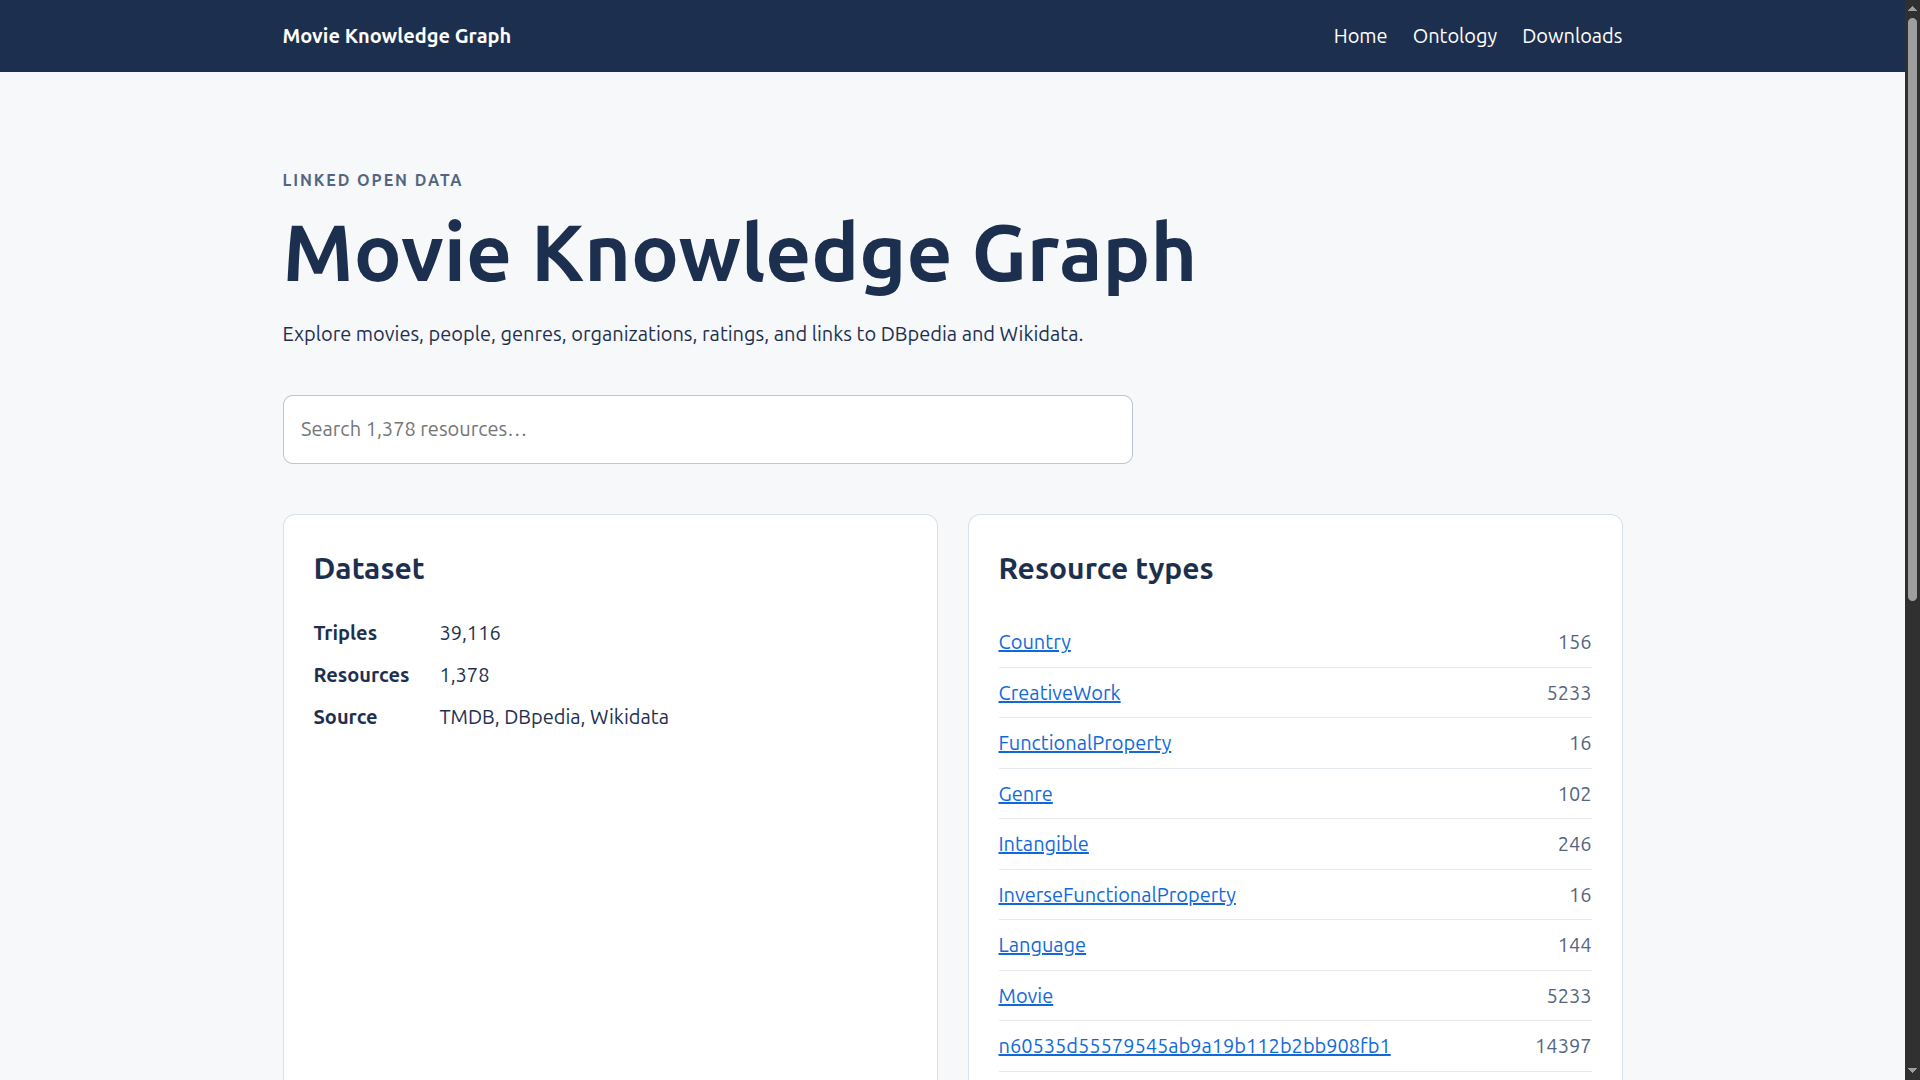
\includegraphics[width=0.82\linewidth]{images/homepage.png}
    \caption{Homepage of the generated static movie knowledge graph browser.}
    \label{fig:appendix-home}
\end{figure}

The ontology page lists the classes and properties extracted from the OWL
file, providing a compact vocabulary browser (Figure~\ref{fig:appendix-ontology}).
The generated resource pages expose canonical URIs, RDF types, and property
values; Figure~\ref{fig:appendix-resource} shows a representative movie page
for Spider-Man: Brand New Day. Finally, the downloads page makes the inferred
graph, raw movie graph, entity links, and ontology available as source files,
as shown in Figure~\ref{fig:appendix-downloads}.

\begin{figure}[!htbp]
    \centering
    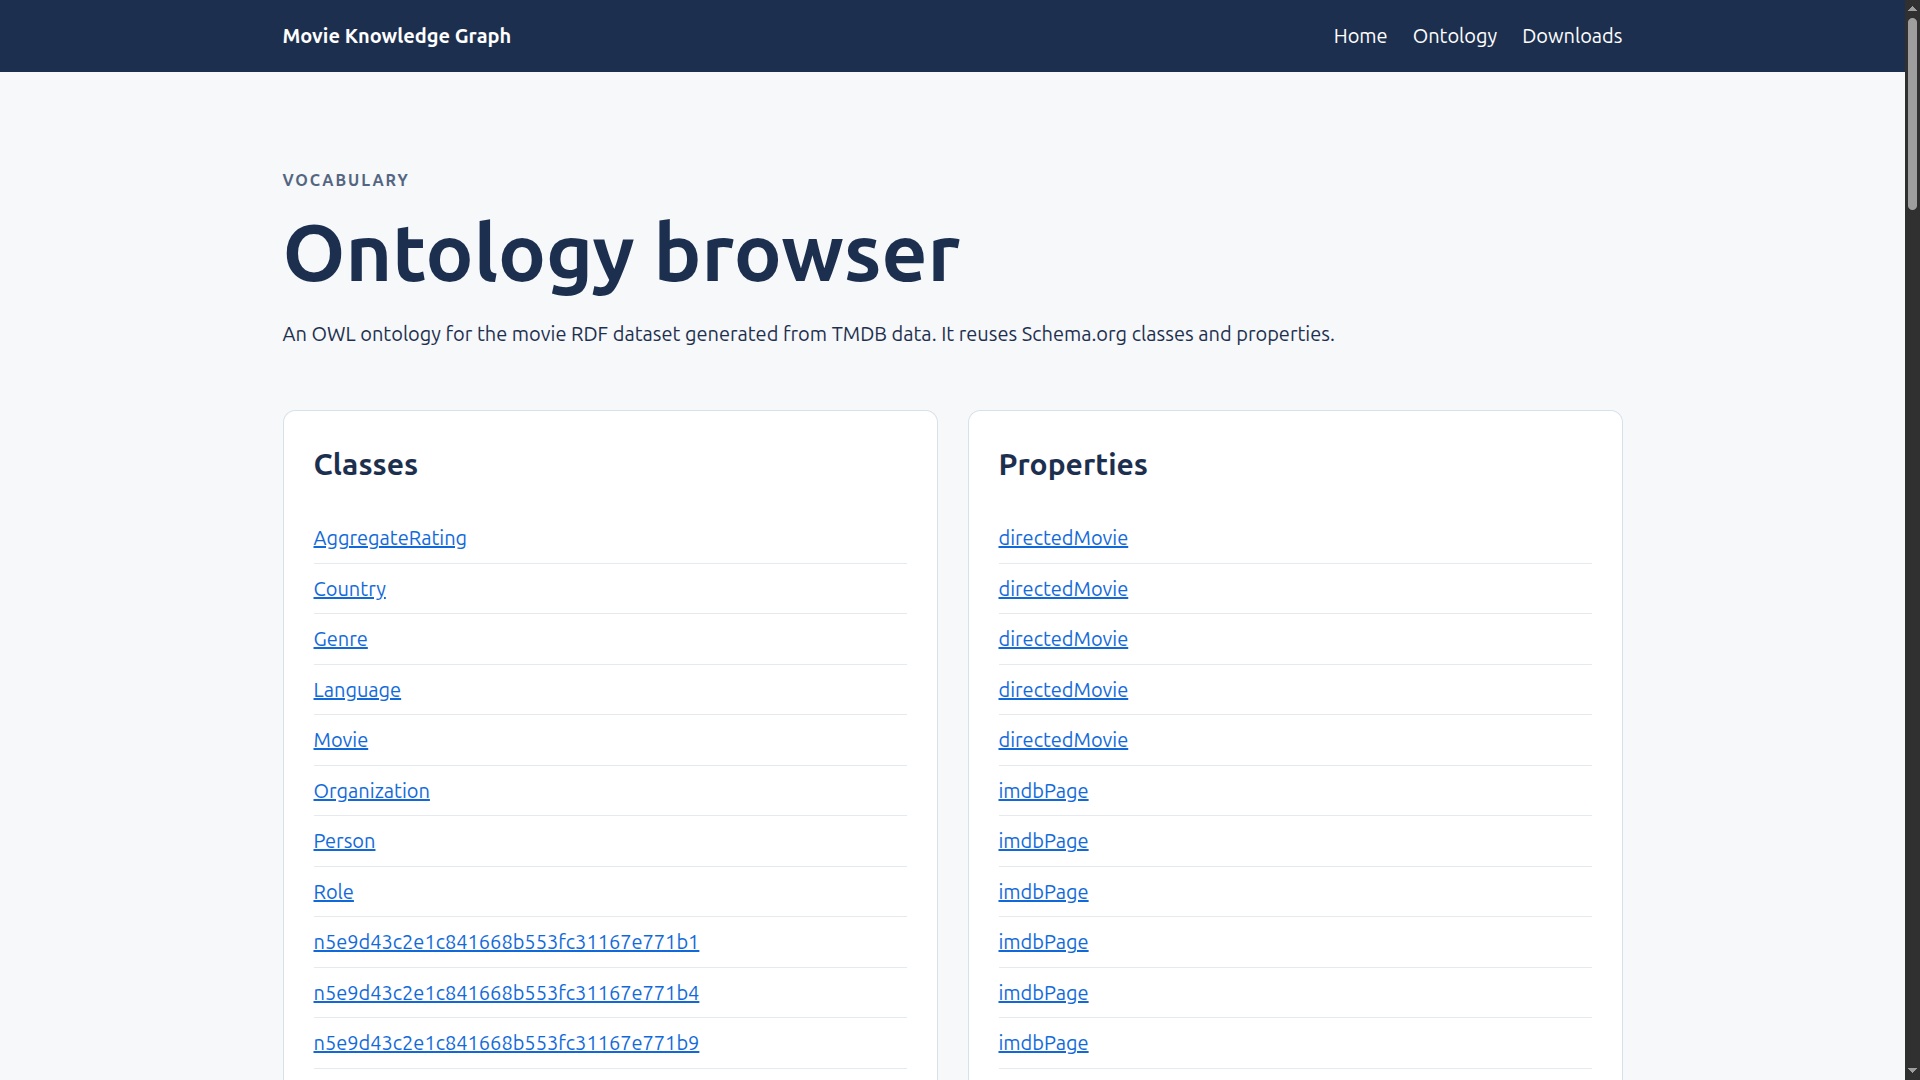
\includegraphics[width=0.82\linewidth]{images/ontology_page.png}
    \caption{Generated ontology browser listing classes and properties.}
    \label{fig:appendix-ontology}
\end{figure}

\begin{figure}[!htbp]
    \centering
    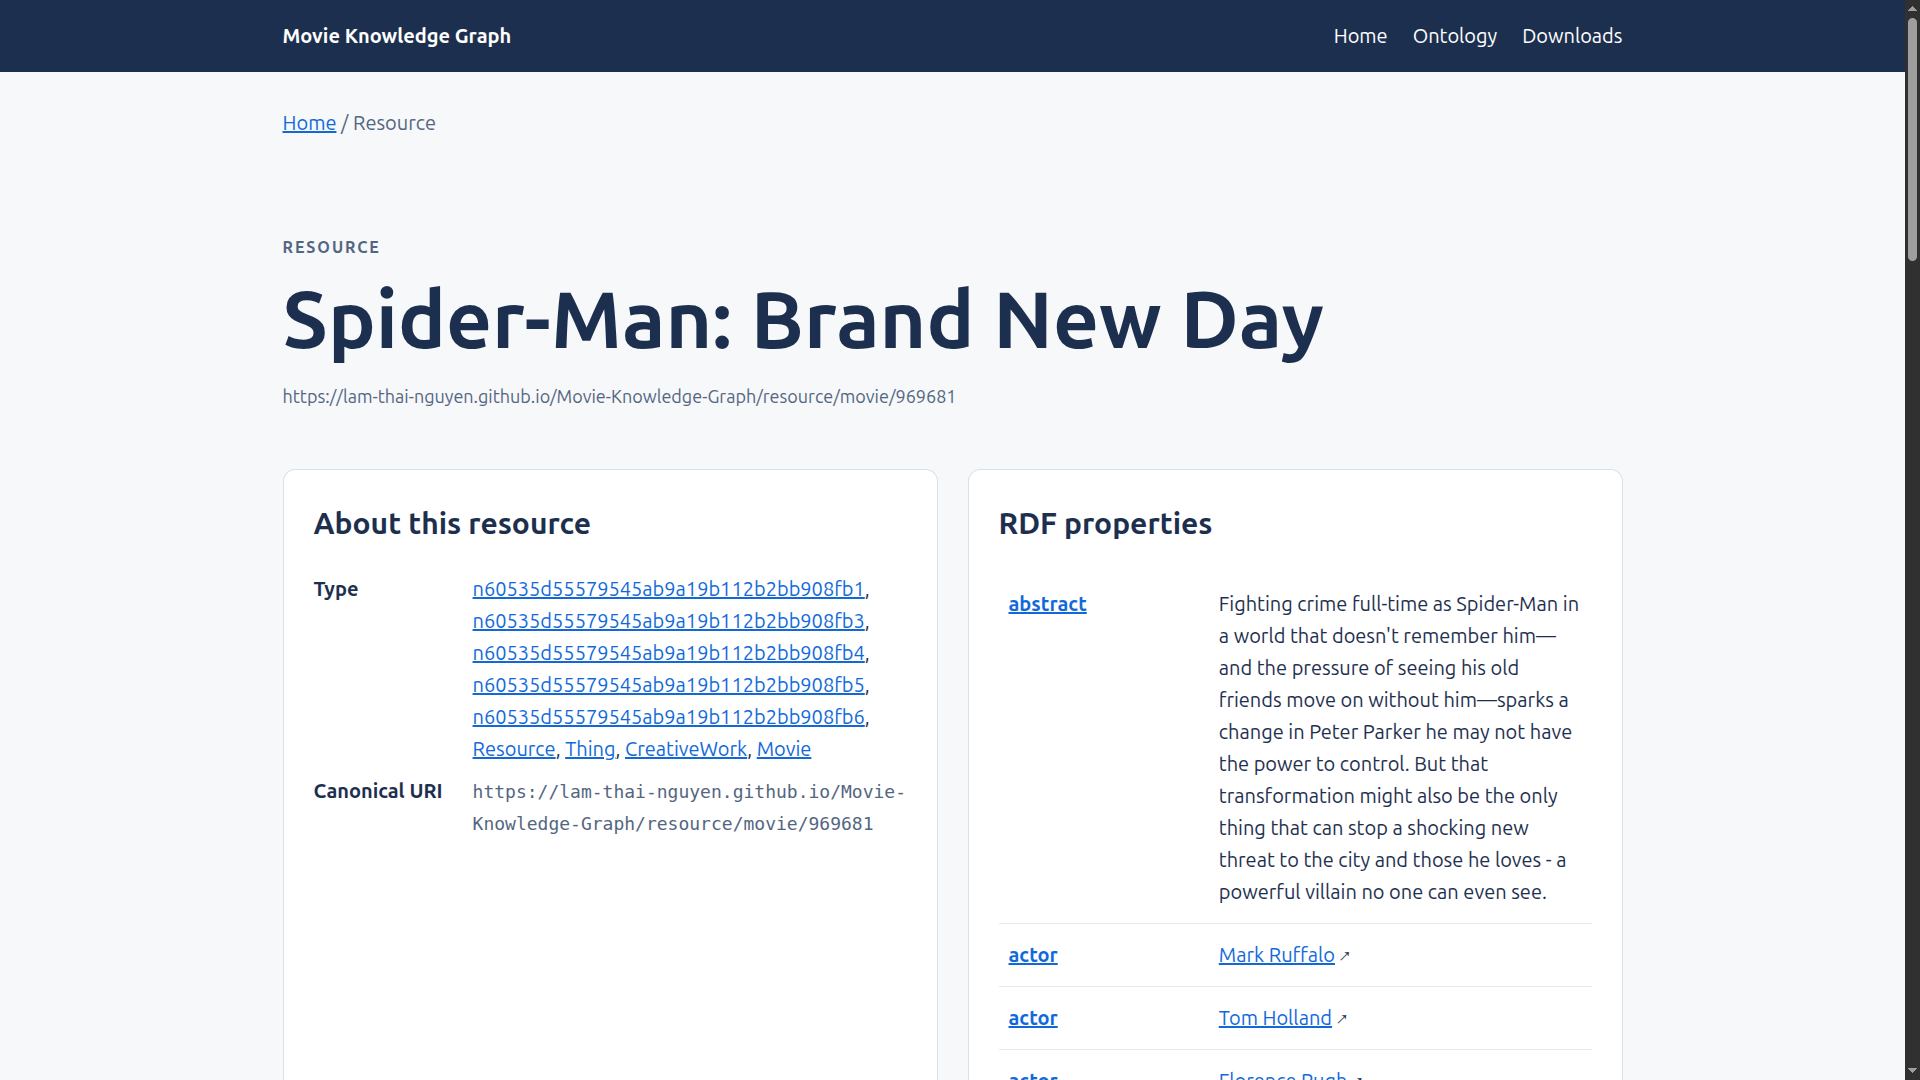
\includegraphics[width=0.82\linewidth]{images/example_search_page.png}
    \caption{Representative generated resource page with its canonical URI and RDF properties.}
    \label{fig:appendix-resource}
\end{figure}

\begin{figure}[!htbp]
    \centering
    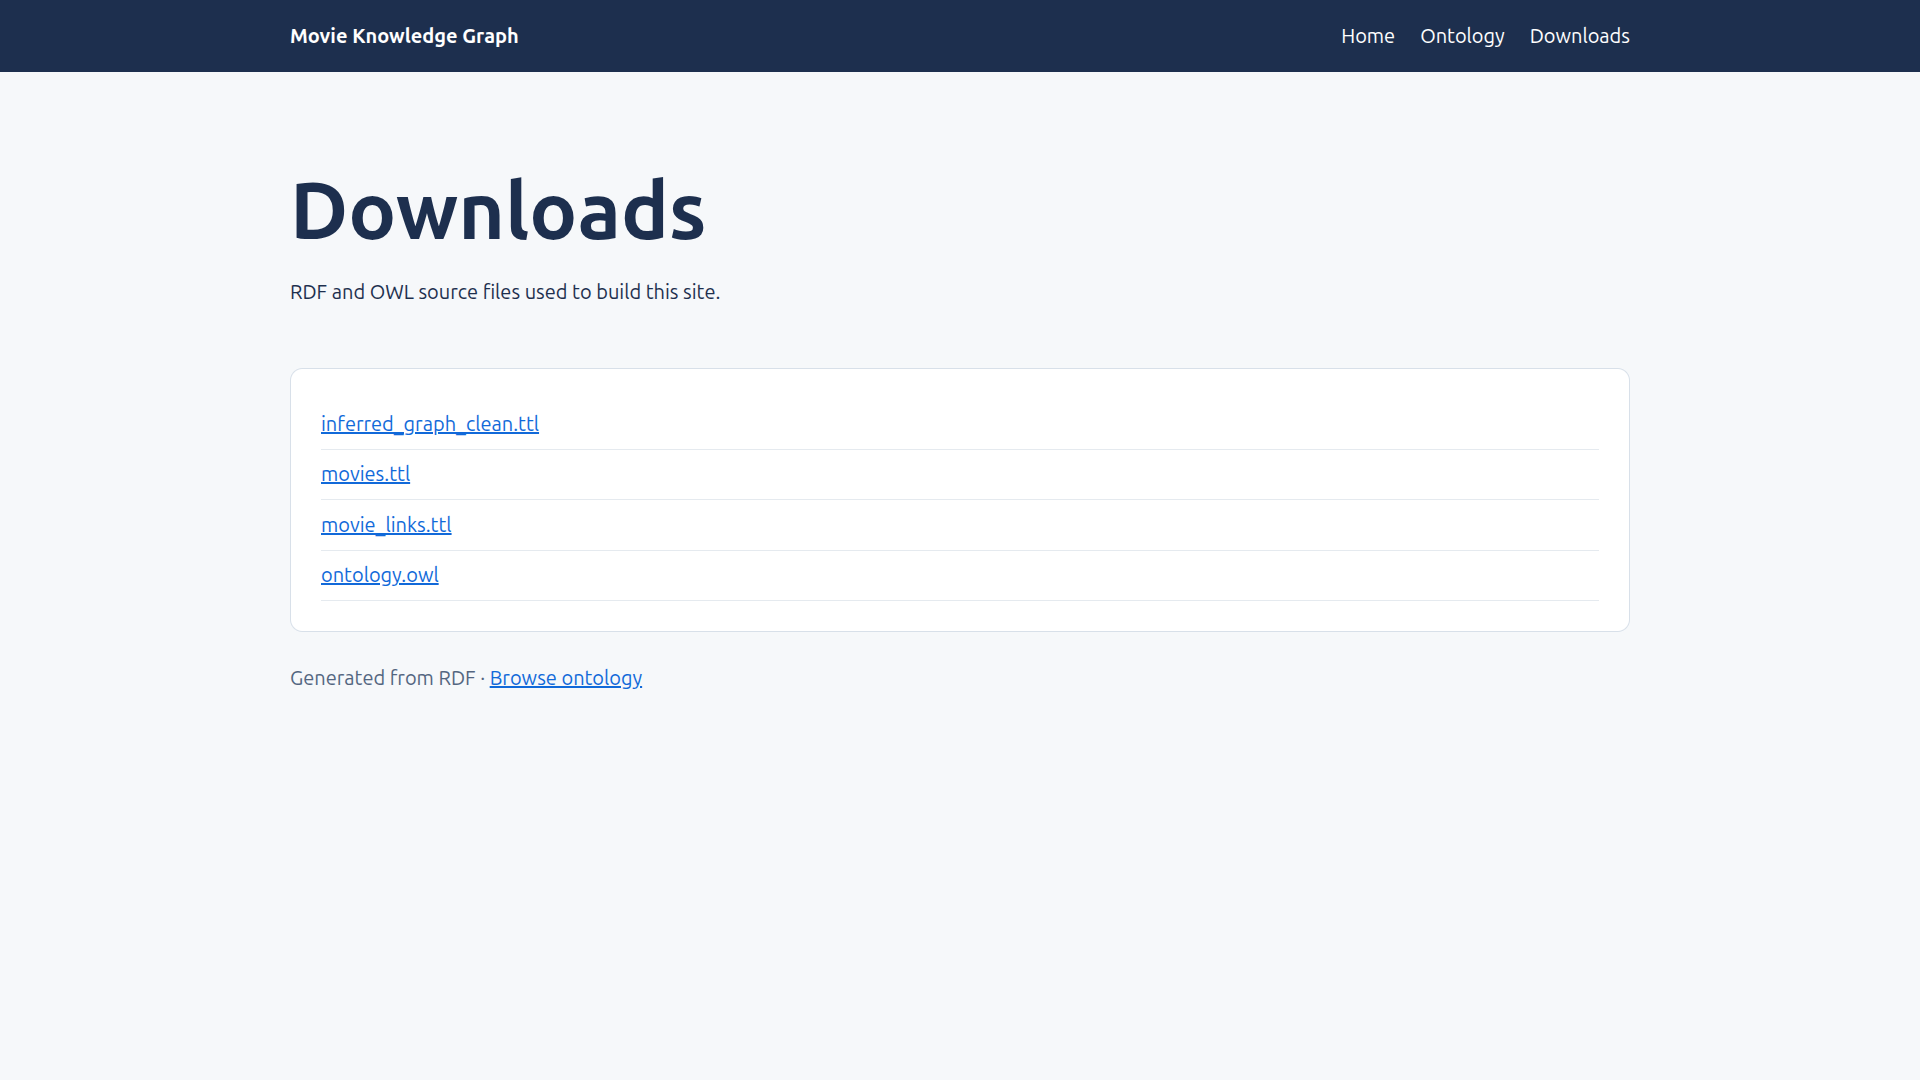
\includegraphics[width=0.82\linewidth]{images/download_page.png}
    \caption{Download page exposing the RDF, links, and OWL source files.}
    \label{fig:appendix-downloads}
\end{figure}